\documentclass[11pt,letterpaper]{article}

% ── Packages ─────────────────────────────────────────────────────────────────
\usepackage[margin=1in]{geometry}
\usepackage{amsmath,amssymb,amsthm}
\usepackage{mathtools}
\usepackage{listings}
\usepackage{xcolor}
\usepackage{hyperref}
\usepackage{booktabs}
\usepackage{tabularx}
\usepackage{longtable}
\usepackage{enumitem}
\usepackage{fancyhdr}
\usepackage{microtype}
\usepackage{lmodern}
\usepackage[T1]{fontenc}
\usepackage{tcolorbox}
\usepackage{tikz}
\usetikzlibrary{arrows.meta,positioning,shapes.geometric,fit,backgrounds}

% ── Hyperref ─────────────────────────────────────────────────────────────────
\hypersetup{colorlinks=true,linkcolor=blue!60!black,urlcolor=blue!60!black}

% ── Header / Footer ──────────────────────────────────────────────────────────
\pagestyle{fancy}\fancyhf{}
\lhead{\small Mirror, Dissonance, Phase}
\rhead{\small Citizen Gardens, Multiplicity Foundation, 2026}
\cfoot{\small\thepage}
\renewcommand{\headrulewidth}{0.4pt}

% ── Theorem environments ──────────────────────────────────────────────────────
\newtheorem{theorem}{Theorem}[section]
\newtheorem{proposition}[theorem]{Proposition}
\newtheorem{definition}[theorem]{Definition}
\newtheorem{corollary}[theorem]{Corollary}
\newtheorem{lemma}[theorem]{Lemma}
\theoremstyle{remark}
\newtheorem{remark}[theorem]{Remark}
\newtheorem{example}[theorem]{Example}

% ── Code listing ─────────────────────────────────────────────────────────────
\definecolor{codebg}{HTML}{F8F8F8}
\definecolor{codeframe}{HTML}{CCCCCC}
\definecolor{kwcolor}{HTML}{0000AA}
\definecolor{cmtcolor}{HTML}{006600}
\lstset{
  backgroundcolor=\color{codebg},frame=single,
  rulecolor=\color{codeframe},
  basicstyle=\ttfamily\footnotesize,
  keywordstyle=\color{kwcolor}\bfseries,
  commentstyle=\color{cmtcolor}\itshape,
  breaklines=true,tabsize=2,showstringspaces=false,captionpos=b
}

% ── Callout boxes ─────────────────────────────────────────────────────────────
\tcbuselibrary{skins,breakable}
\newtcolorbox{oraclebox}[1]{
  colback=blue!4!white,colframe=blue!40!black,
  fonttitle=\bfseries,title=#1
}
\newtcolorbox{tensionbox}[1]{
  colback=orange!5!white,colframe=orange!50!black,
  fonttitle=\bfseries,title=#1
}
\newtcolorbox{precisionbox}{
  colback=green!4!white,colframe=green!40!black,
  fonttitle=\bfseries,title=Precision Question
}

% ── Math operators ────────────────────────────────────────────────────────────
\newcommand{\pmd}{\textsc{pmd}}
\newcommand{\rhogate}{\rho_{\mathrm{gate}}}
\newcommand{\rhosys}{\rho}

% ─────────────────────────────────────────────────────────────────────────────
\title{%
  \textbf{Mirror, Dissonance, Phase:}\\[4pt]
  \large A Governance Oracle for Agentic Systems\\[8pt]
  \normalsize\textit{Defensive Publication --- Prior Art Disclosure}\\
  \normalsize\textit{Paper C in the Phase Mirror Publication Series}
}
\author{%
  Citizen Gardens\\
  \small The Foundation of Multiplicity\\
  \small \texttt{github.com/MultiplicityTheory/PhaseMirror}
}
\date{April 26, 2026}

% =============================================================================
\begin{document}
\maketitle\thispagestyle{fancy}

\begin{abstract}
We describe the \emph{Phase Mirror Dissonance} (\pmd{}) loop as a callable,
auditable governance oracle for agentic AI systems.  Unlike prior work that
treats safety as a model property or a runtime filter, \pmd{} treats
\emph{governance itself} as a versioned, auditable artifact that can be
called over any structured input --- a repository, a pull request, a CI
configuration, a policy document, or a legal workflow --- and that always
returns three things: a dissonance list, a set of actionable levers
(each with an owner, metric, and horizon), and a precision question that
names the deepest unresolved assumption in the current state.  We formalize
the \pmd{} operating loop, define six canonical dissonance patterns for
agentic AI deployments (autonomy vs.\ governance, compliance vs.\ accuracy,
velocity vs.\ safety, open-core vs.\ proprietary, local vs.\ cloud,
L0-immutability vs.\ evolvability), and describe how the oracle is
implemented as a build-time component that feeds dissonance reports as
JSON into CI/CD pipelines and pull request checks.  As a case study we
describe the application of this methodology to legal AI governance,
mapping output confidence tiers to liability-graded documentation and
review requirements without constituting legal advice.  This document
constitutes a defensive publication placing the described governance
\emph{method} in the public domain as prior art.
\end{abstract}

\tableofcontents\newpage

% =============================================================================
\section{Introduction: Why Governance Needs an Oracle}
% =============================================================================

Current approaches to AI governance divide roughly into two families.  The
first treats safety as a \emph{model property} --- a fine-tuning objective,
a refusal classifier, or a RLHF preference --- that is baked into model
weights before deployment.  The second treats safety as a \emph{runtime
filter} --- a post-generation classifier or a guardrail layer that rejects
outputs after the fact.  Both families share a common limitation: governance
is \emph{implicit and non-auditable}.  Neither produces a signed, versioned
record of \emph{which} governance rules were active, \emph{which} tensions
they resolved, and \emph{what} the system chose to prioritize when the rules
conflicted.

Agentic AI systems --- systems that plan over sequences of tool calls,
write and execute code, modify repositories, and take consequential actions
--- demand a third family: governance as an \emph{auditable oracle}.

An oracle in this sense is a component that:
\begin{enumerate}[leftmargin=1.5em]
  \item Accepts a structured payload (an expression, a state transition,
        a repository scan, or a policy artifact).
  \item Evaluates it against a versioned, immutable ruleset.
  \item Returns a deterministic, signed report containing a dissonance
        score, a decision (\texttt{PASS}/\texttt{FAIL}), and a structured
        list of tensions and levers.
  \item Writes an append-only audit entry regardless of the decision.
\end{enumerate}

The Phase Mirror Dissonance (\pmd{}) system, developed under the
Multiplicity Foundation and publicly versioned at
\href{https://github.com/MultiplicityTheory/PhaseMirror-HQ}%
{\texttt{MultiplicityTheory/PhaseMirror-HQ}}, is a concrete implementation
of this oracle pattern.

\subsection{What This Paper Freezes as Prior Art}

This paper places the following \emph{method} in the public domain:

\begin{itemize}[leftmargin=1.5em]
  \item Treating a governance method (not a model or runtime) as a
        callable, auditable oracle that produces a dissonance list,
        actionable levers, and a precision question.
  \item Using this oracle to manage canonical tensions in agentic AI
        deployments (Section~\ref{sec:patterns}).
  \item Applying this oracle specifically to legal AI governance with
        explicit mapping from output confidence tiers to documentation
        and review tiers (Section~\ref{sec:legal}).
  \item Positioning the oracle as a build-time artifact that feeds CI/CD
        pipelines rather than a runtime layer (Section~\ref{sec:impl}).
  \item The open-core licensing structure in which the oracle \emph{method}
        is public but the managed service delivery is license-restricted
        (Section~\ref{sec:business}).
\end{itemize}

% =============================================================================
\section{The PMD Operating Loop}
\label{sec:loop}
% =============================================================================

\subsection{Formal Definition}

\begin{definition}[PMD Operating Loop]
\label{def:pmd-loop}
The \emph{Phase Mirror Dissonance operating loop} is a six-step cycle
$\mathcal{L} = (I, E, D, R, A, W)$:

\begin{enumerate}[leftmargin=1.5em, label=\textbf{Step \arabic*.}]
  \item \textbf{Ingest} ($I$): Accept a structured payload $e$ of type
        $\tau \in \{\texttt{ExpressionPayload}, \texttt{StateTransitionPayload},
        \texttt{ArtifactScan}\}$.
  \item \textbf{Evaluate} ($E$): Run the scorer registry $\mathcal{S}_\tau$
        against $e$; compute dissonance $\rhosys(e) = \sum_i w_i \cdot s_i(e)$
        clamped to $[0, 2]$.
  \item \textbf{Decide} ($D$): Gate on $\rhogate = 1.0$:
        $\texttt{execute} \Leftrightarrow \rhosys < \rhogate$.
        Identify auto-fail conditions.
  \item \textbf{Report} ($R$): Construct a \texttt{DissonanceReport}
        containing: decision, $\rhosys$, margin, tensions list,
        suppressed tensions, and metadata.
  \item \textbf{Act} ($A$): Surface actionable levers: for each tension
        $t_i$, produce a triple
        $(\texttt{owner}_i, \texttt{metric}_i, \texttt{horizon}_i)$.
  \item \textbf{Write} ($W$): Append the report to the \texttt{AuditLedger}
        \emph{unconditionally}, regardless of the decision.
\end{enumerate}
\end{definition}

\begin{oraclebox}{The PMD Oracle Output Contract}
Every call to the oracle produces \emph{exactly three things}:
\begin{itemize}[leftmargin=1em]
  \item A \textbf{dissonance list}: named tensions with severity, weight,
        and margin.
  \item A \textbf{lever set}: at least one
        $(\texttt{owner}, \texttt{metric}, \texttt{horizon})$ triple per
        active tension.
  \item A \textbf{precision question}: one question that names the deepest
        unresolved assumption in the current evaluation context.
\end{itemize}
\end{oraclebox}

\subsection{Communication Constraints}

The \pmd{} loop is designed to be \emph{legible under adversarial load}.
Three communication constraints are enforced on all oracle outputs:

\begin{enumerate}[leftmargin=1.5em]
  \item \textbf{Short}: No tension summary exceeds one sentence.
        No lever description exceeds one line.
  \item \textbf{Neutral}: Tension descriptions name conditions, not
        judgments.  ``Rollback trigger detected'' not ``Dangerous state
        change attempted.''
  \item \textbf{Non-moralizing}: The oracle does not infer intent.
        It reports structural violations.  The precision question
        may name an assumption about intent, but never attributes it.
\end{enumerate}

These constraints are not stylistic preferences.  They are necessary for
the oracle to remain trustworthy in adversarial conditions: a governance
system that moralizes can be gamed by aligning its rhetoric; one that
names structural conditions cannot.

\subsection{The Precision Question Protocol}

The precision question is the oracle's most distinctive output.  It is
produced by the orchestration layer (not the evaluation engine) after
the dissonance report is constructed, and it names a hidden assumption
that the report does not resolve.

\begin{example}[Precision Question Instances]
\label{ex:precision}
\begin{itemize}[leftmargin=1.5em]
  \item When \texttt{compliance\_vs\_accuracy} tension fires:
        ``Are we optimizing for compliance or accuracy in this deployment
        context?  They cannot be simultaneously maximized at the current
        scorer weights.''
  \item When \texttt{rollback\_trigger\_active} tension fires at $\rhosys = 0.9$
        (below gate):
        ``Is the rollback trigger here an emergency signal or a test artifact?
        The oracle cannot distinguish them; the audit ledger will record which
        assumption was made.''
  \item When \texttt{governance\_version\_mismatch} fires during a canary
        rollout: ``Which version of the governance constitution should govern
        the canary population: the incoming version it is testing, or the
        stable version it is replacing?''
\end{itemize}
\end{example}

% =============================================================================
\section{Canonical Dissonance Patterns for Agentic AI}
\label{sec:patterns}
% =============================================================================

Six canonical tension patterns appear repeatedly in agentic AI deployments.
The \pmd{} oracle maps each pattern to a named dissonance signal, a scorer
weight, a default owner, and a recommended horizon for resolution.

\begin{longtable}{p{2.8cm}p{3.2cm}p{1.4cm}p{2.4cm}p{2.4cm}}
\caption{Canonical Agentic Dissonance Patterns}
\label{tab:patterns}\\
\toprule
\textbf{Tension} & \textbf{Signal ID(s)} & \textbf{$w_i$} &
\textbf{Default Owner} & \textbf{Horizon} \\
\midrule
\endfirsthead
\toprule
\textbf{Tension} & \textbf{Signal ID(s)} & \textbf{$w_i$} &
\textbf{Default Owner} & \textbf{Horizon} \\
\midrule
\endhead
\midrule
\multicolumn{5}{r}{\small\textit{Continued on next page}}\\
\endfoot
\bottomrule
\endlastfoot
%
Autonomy vs.\ governance
  & \texttt{unauthorized\_prime\_index},
    \texttt{contractivity\_assertion\_absent}
  & 0.3, 0.4
  & Governance Lead
  & 7 days \\[4pt]
%
Compliance vs.\ accuracy
  & \texttt{governance\_version\_mismatch},
    \texttt{semantic\_drift}
  & 0.2, 0.3
  & Product + Legal
  & 30 days \\[4pt]
%
Velocity vs.\ safety
  & \texttt{stale\_base\_disabled},
    \texttt{rollback\_trigger\_active}
  & 0.3, 0.5
  & SRE Lead
  & 7 days \\[4pt]
%
Open-core vs.\ proprietary
  & \texttt{boundary\_absent}
  & 0.3
  & Business / Licensing
  & 90 days \\[4pt]
%
Local vs.\ cloud
  & \texttt{twin\_desynced}
  & 0.4
  & Infrastructure
  & 30 days \\[4pt]
%
L0-immutability vs.\ evolvability
  & \texttt{bad\_precedent},
    \texttt{immutable\_path\_access}
  & 0.5, 0.7
  & Constitutional Core
  & 90 days \\
\end{longtable}

\subsection{Pattern Detail: Autonomy vs.\ Governance}

\begin{tensionbox}{Autonomy vs.\ Governance}
\textbf{Core question:} How much decision authority can an agent exercise
before it must surface a dissonance to its governance layer?

\textbf{Manifestation:} An agent expression claims a prime index that is
not in the authorized set, or lacks a contractivity assertion that would
bound its action space.

\textbf{Lever:} Reduce the authorized prime index ceiling
(\texttt{MAX\_PRIME\_INDEX}); require contractivity markers in all
agent expressions; gate on failing harness vectors.

\textbf{Horizon:} 7 days (operational SLO).
\end{tensionbox}

This tension is the deepest in the \pmd{} framework because it is
self-referential: the governance oracle itself operates at a prime index,
and any agent that successfully overrides its own prime index has escaped
the governance layer.  The contractivity bound $\kappa(p) = p/(p+1)$
provides the formal mechanism for containing this: no agent operating at
prime index $p$ can produce a fixed-point contraction ratio exceeding
$p/(p+1) < 1$, which means the governance attractor is always reachable.

\subsection{Pattern Detail: Compliance vs.\ Accuracy}

\begin{tensionbox}{Compliance vs.\ Accuracy}
\textbf{Core question:} When a governance version update changes the
required output format or constraints, which version governs in-flight
requests?

\textbf{Manifestation:} An output expression's \texttt{governance\_version}
tag does not match the current runtime epoch.  Or a semantically accurate
output is token-disjoint from the governing input, triggering
\texttt{semantic\_drift}.

\textbf{Lever:} Explicit governance version pinning at session start;
semantic drift threshold tuning; canary rollout of new governance versions
before full adoption.

\textbf{Horizon:} 30 days (product release cycle).
\end{tensionbox}

\subsection{Pattern Detail: Velocity vs.\ Safety}

\begin{tensionbox}{Velocity vs.\ Safety}
\textbf{Core question:} When a rollback trigger is active, does the system
proceed with a degraded but fast path, or pause for governance approval?

\textbf{Manifestation:} \texttt{rollback\_trigger\_active} fires at weight
0.5, combined with \texttt{stale\_base\_disabled} (0.3), produces
$\rhosys = 0.8$ --- below the kill-switch gate but above the monitoring
threshold $\rhostar = 0.7$.

\textbf{Lever:} Require explicit operator acknowledgment when
$\rhosys \in [\rhostar, \rhogate)$; log all ``below gate but above
monitoring'' decisions to the audit ledger with a mandatory precision
question.

\textbf{Horizon:} 7 days (incident response cycle).
\end{tensionbox}

\subsection{Pattern Detail: L0-Immutability vs.\ Evolvability}

This is the highest-weight tension in the registry.  Any state transition
that targets an immutable path (\texttt{policy/phase\_mirror/},
\texttt{contracts/system\_invariants.yaml}) is assigned $w = 0.7$,
ensuring that a single such event reaches $\rhosys = 0.7 = \rhostar$
(monitoring threshold) and that two events reach $\rhosys = 1.4$,
well past the kill-switch gate.

The L0/L1 distinction is central here:

\begin{definition}[L0 and L1 Invariants]
\label{def:l0l1}
\textbf{L0 invariants} are non-negotiable constitutional constraints
that no governance evolution can remove.  In the reference implementation
these include: (i) every evaluation writes to the audit ledger; (ii) the
kill-switch gate is always active; (iii) immutable paths cannot be
modified by any agentic expression.

\textbf{L1 invariants} are strong defaults that can be overridden by
an authorized governance evolution process, subject to ADR review
and council sign-off.  L1 rules include scorer weights, threshold
values, and domain-separation info strings.
\end{definition}

This distinction allows the \pmd{} oracle to evolve its L1 rule surface
(e.g., adjusting scorer weights in response to deployment experience)
without compromising the L0 guarantees that make the audit ledger
trustworthy.

% =============================================================================
\section{Governance Oracle Implementation}
\label{sec:impl}
% =============================================================================

\subsection{Build-Time vs.\ Runtime Oracle Positioning}

The \pmd{} oracle is designed as a \emph{build-time} governance component,
not a runtime safety filter.  This distinction is consequential:

\begin{center}
\begin{tabular}{lll}
\toprule
\textbf{Property} & \textbf{Build-time oracle} & \textbf{Runtime filter} \\
\midrule
Invocation point  & CI/CD, PR check, tag gate & Post-generation, pre-user \\
Input artifacts   & Repos, configs, policies   & Model output tokens \\
Output            & JSON report + audit entry  & Pass/reject decision \\
Auditability      & Full ledger, immutable     & Usually ephemeral \\
Versioning        & Governance version tag     & Model version \\
Failure mode      & Block merge/deploy         & Reject response \\
\bottomrule
\end{tabular}
\end{center}

\subsection{JSON Dissonance Report Schema}

The oracle produces a JSON report that feeds directly into PR checks
and CI gates.  The wire schema (per ADR-015) is:

\begin{lstlisting}[language=Python, caption={%
  DissonanceReport wire schema (ADR-015)}]
{
  "execute":         true | false,
  "safe":            true | false,   // always == execute
  "rho":             0.0,            // dissonance score
  "rho_star":        0.7,            // monitoring threshold
  "kappa_min":       0.3,            // minimum contractivity
  "rho_threshold":   1.0,            // kill-switch gate
  "margin_to_fail":  1.0,            // rho_threshold - rho
  "threshold_state": "below_threshold" | "at_or_above_threshold",
  "decision":        "PASS" | "FAIL",
  "tensions": [
    {
      "signal_id":  "contractivity_assertion_absent",
      "severity":   "high",
      "summary":    "Expression lacks contractivity markers."
    }
  ],
  "suppressed_tensions": [...],
  "metadata": {
    "rollback_trigger": "none",
    "mode":             "expression",
    "payload_type":     "ExpressionPayload"
  }
}
\end{lstlisting}

\subsection{CI/CD Integration Pattern}

\begin{figure}[h]
\centering
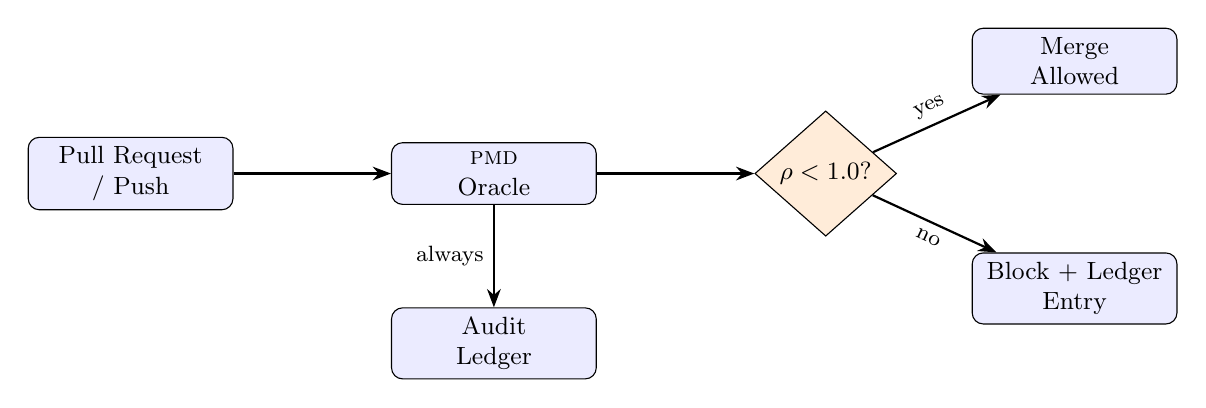
\begin{tikzpicture}[
  node distance=1.2cm and 2.0cm,
  every node/.style={font=\small},
  box/.style={draw,rounded corners,minimum width=2.6cm,
              minimum height=0.7cm,align=center,fill=blue!8},
  gate/.style={draw,diamond,minimum width=1.8cm,minimum height=0.7cm,
               inner sep=1pt,align=center,fill=orange!15},
  arr/.style={-{Stealth},thick}
]
\node[box]  (pr)      {Pull Request\\/ Push};
\node[box,right=of pr]  (scan)    {\pmd{}\\Oracle};
\node[gate,right=of scan] (gate)  {$\rhosys < 1.0$?};
\node[box,above right=0.6cm and 1.4cm of gate]  (pass)
                                  {Merge\\Allowed};
\node[box,below right=0.6cm and 1.4cm of gate]  (fail)
                                  {Block + Ledger\\Entry};
\node[box,below=1.3cm of scan]    (ledger)  {Audit\\Ledger};

\draw[arr] (pr) -- (scan);
\draw[arr] (scan) -- (gate);
\draw[arr] (gate) -- node[above,sloped]{\footnotesize yes} (pass);
\draw[arr] (gate) -- node[below,sloped]{\footnotesize no}  (fail);
\draw[arr] (scan) -- (ledger) node[midway,left]{\footnotesize always};
\end{tikzpicture}
\caption{PMD oracle as a CI/CD gate.  The audit ledger receives an entry
on every evaluation, regardless of the gate decision.}
\label{fig:cicd}
\end{figure}

The CLI package \texttt{@phase-mirror/cli} provides this integration:

\begin{lstlisting}[language=bash, caption={%
  PR check usage of @phase-mirror/cli}]
# In .github/workflows/governance.yml
- name: Phase Mirror governance check
  run: |
    phase-mirror analyze \
      --input-text  "${{ github.event.pull_request.title }}" \
      --output-expr "${{ steps.generate.outputs.expr }}" \
      --repo-root   "${{ github.workspace }}" \
      --ledger-path "${{ github.workspace }}/state/ledger.json"
  # Exit code: 0=PASS, 1=FAIL, 2=REVIEW, 3=error
\end{lstlisting}

\subsection{L0 Policy-as-Code}

The L0 invariants are encoded as a Python module
(\texttt{governance/policy/phase\_mirror/}), not as configuration
or comments.  This means they are:

\begin{itemize}[leftmargin=1.5em]
  \item \textbf{Version-controlled}: Every change is a diff, reviewed
        via PR, and tagged with a governance version string.
  \item \textbf{Tested}: The golden-vector harness validates all L0
        behaviors on every commit.
  \item \textbf{Immutable at the path level}: Any state transition
        targeting the policy path fires the
        \texttt{immutable\_path\_access} scorer ($w = 0.7$).
  \item \textbf{Callable}: Any downstream component can call
        \texttt{evaluate()} and receive a signed report.
\end{itemize}

The L1 rules --- scorer weights, threshold values, domain-separation
strings --- are encoded in \texttt{governance/policy/tension\_policy.py}
and governed by ADR review.  They can be updated without modifying the
L0 evaluation engine.

% =============================================================================
\section{Case Study: Legal AI Governance}
\label{sec:legal}
% =============================================================================

\textit{Note: This section describes a governance method case study.
It does not constitute legal advice.  The tier definitions and
confidence mappings described here are governance design patterns,
not legal standards.}

\subsection{Problem Statement}

Legal organizations deploying AI assistants face a structural tension
that the \pmd{} framework is well-suited to formalize: \emph{output
confidence cannot be directly observed, but liability exposure is
real and tiered}.  A legal AI that is 72\% confident in a citation
carries different review obligations than one that is 97\% confident,
but without a governance oracle, there is no systematic mechanism to
route those outputs to the appropriate review tier.

The \pmd{} framework addresses this by treating confidence scores as
inputs to a specialized scorer registry and mapping the resulting
dissonance to documentation and review requirements.

\subsection{Confidence-to-Liability Tier Mapping}

\begin{definition}[Legal Confidence Tier]
\label{def:legal-tier}
A \emph{legal confidence tier} $\mathcal{T}(c)$ is assigned based on the
output confidence score $c \in [0,1]$:
\[
  \mathcal{T}(c) = \begin{cases}
    \text{Tier A: Autonomous}   & c \geq 0.95, \\
    \text{Tier B: Supervised}   & 0.80 \leq c < 0.95, \\
    \text{Tier C: Reviewed}     & 0.65 \leq c < 0.80, \\
    \text{Tier D: Blocked}      & c < 0.65.
  \end{cases}
\]
\end{definition}

Each tier maps to a governance lever set:

\begin{center}
\begin{tabular}{p{1.5cm}p{2.6cm}p{2.6cm}p{3.4cm}p{1.8cm}}
\toprule
\textbf{Tier} & \textbf{Documentation} & \textbf{Review} &
\textbf{PMD Signal} & \textbf{Horizon} \\
\midrule
A & Auto-generated log entry & None required &
  $\rhosys < \rhostar = 0.7$ & Continuous \\
B & Structured summary + confidence trace &
  Spot-check 10\% &
  $\rhosys \in [0.7, 0.85)$ & 24 hours \\
C & Full reasoning trace + citation list &
  Attorney review before use &
  $\rhosys \in [0.85, 1.0)$ & 48 hours \\
D & Blocked; reasoning trace retained &
  Escalate + PMD audit entry &
  $\rhosys \geq 1.0$ & Immediate \\
\bottomrule
\end{tabular}
\end{center}

\subsection{Legal Dissonance Scorers}

The legal governance application extends the base scorer registry with
domain-specific signals:

\begin{center}
\begin{tabular}{lll}
\toprule
\textbf{Signal ID} & \textbf{Weight} & \textbf{Condition} \\
\midrule
\texttt{citation\_confidence\_low}   & 0.35 &
  $c_{\text{citation}} < 0.80$ \\
\texttt{jurisdiction\_absent}        & 0.25 &
  No jurisdiction tag in output expression \\
\texttt{precedent\_conflict}         & 0.40 &
  Output cites conflicting precedents \\
\texttt{date\_staleness}             & 0.20 &
  Cited source older than governance horizon \\
\texttt{verbatim\_statute}           & 0.30 &
  Output contains verbatim statutory text
  without attribution \\
\texttt{liability\_floor\_absent}    & 0.40 &
  No liability-floor marker in expression body \\
\bottomrule
\end{tabular}
\end{center}

\begin{example}[Legal Governance Oracle Call]
A legal AI assistant generates a research memo claiming to cite
\textit{Roe v.\ Wade} in a jurisdiction where the precedent has been
superseded.  The oracle fires:
\begin{itemize}[leftmargin=1.5em]
  \item \texttt{precedent\_conflict} ($w = 0.40$): the cited case is
        in conflict with current binding authority.
  \item \texttt{date\_staleness} ($w = 0.20$): the source predates the
        governance horizon by more than the configured window.
  \item \texttt{liability\_floor\_absent} ($w = 0.40$): the memo body
        contains no liability-floor marker.
\end{itemize}
Total: $\rhosys = 0.40 + 0.20 + 0.40 = 1.00 = \rhogate$.  Decision:
\texttt{FAIL}.  The oracle blocks the output, writes a ledger entry,
and surfaces the precision question:

\begin{precisionbox}
``Is the current binding authority in the target jurisdiction configured
in the governance version active at the time of this query?
If not, the precedent conflict scorer cannot be trusted to fire correctly.''
\end{precisionbox}

The memo is routed to Tier D: blocked, with reasoning trace retained
for attorney review.
\end{example}

\subsection{Governance Levers for Legal Deployment}

For a legal AI deployment operating under this framework, the standard
lever set per tension is:

\begin{center}
\begin{tabular}{p{3.0cm}p{3.0cm}p{2.2cm}p{2.4cm}}
\toprule
\textbf{Tension} & \textbf{Lever} & \textbf{Owner} & \textbf{Horizon} \\
\midrule
Compliance vs.\ accuracy &
  Governance version pinning to jurisdiction-specific epoch &
  Legal + Governance Lead & 30 days \\
Velocity vs.\ safety &
  Mandatory 48-hour review window for Tier C outputs &
  Practice Group Lead & Continuous \\
Autonomy vs.\ governance &
  Confidence floor at 0.95 for Tier A autonomous use &
  Risk / Compliance & 90 days \\
Precedent freshness &
  Automated citation-date staleness check on all research memos &
  Knowledge Management & 30 days \\
\bottomrule
\end{tabular}
\end{center}

% =============================================================================
\section{Dissonance as a Design Instrument}
\label{sec:design}
% =============================================================================

A key contribution of the \pmd{} framework is treating dissonance not
only as a \emph{gate} but as a \emph{design instrument}.  The margin
to failure $\mu = \rhogate - \rhosys$ is a continuous signal, not a
binary alarm.  Teams that observe $\mu$ trending toward zero across
successive deployments are receiving advance warning of governance
erosion before any individual deployment crosses the threshold.

\begin{definition}[Dissonance Drift]
\label{def:drift}
Let $\{\rhosys^{(t)}\}_{t=1}^{T}$ be the time series of dissonance
scores for a deployment.  \emph{Dissonance drift} is:
\[
  \delta = \frac{1}{T-1} \sum_{t=2}^{T} (\rhosys^{(t)} - \rhosys^{(t-1)}).
\]
$\delta > 0$ indicates systematic governance erosion.
$\delta < 0$ indicates governance tightening.
$\abs{\delta} > \epsilon_{\text{drift}}$ (a configurable threshold)
triggers a governance review regardless of whether any individual
$\rhosys^{(t)}$ has crossed $\rhogate$.
\end{definition}

This makes the \pmd{} oracle an instrument for \emph{proactive} governance:
teams do not wait for a \texttt{FAIL} decision to investigate their
governance posture.  The ledger time series gives them a running estimate
of the trajectory.

\subsection{The Precision Question as a Design Loop}

The precision question protocol (Section~\ref{sec:loop}) closes a feedback
loop that most governance systems leave open.  A standard oracle says
``blocked.''  The \pmd{} oracle says ``blocked, and here is the assumption
you need to resolve before the next call will pass.''  This distinction
is important for agentic systems because agents iterate: they will call
the oracle again.  Giving them a named, unresolved assumption accelerates
convergence toward governance compliance.

\begin{oraclebox}{Design Loop Invariant}
After any \texttt{FAIL} decision, a well-formed response from the
governance-aware agent is:
\begin{enumerate}[leftmargin=1em]
  \item Read the dissonance list.
  \item Answer the precision question explicitly.
  \item Update the expression or state payload accordingly.
  \item Re-invoke the oracle.
\end{enumerate}
If the oracle is working correctly and the precision question was
accurate, the re-invocation will produce a lower $\rhosys$.
\end{oraclebox}

% =============================================================================
\section{Open-Core Positioning and Licensing}
\label{sec:business}
% =============================================================================

The Phase Mirror project is structured as an open-core system.  The
following components are and will remain open-source under a permissive
license:

\begin{itemize}[leftmargin=1.5em]
  \item The \pmd{} evaluation engine
        (\texttt{policy/phase\_mirror/}).
  \item The \texttt{@phase-mirror/cli} standalone analysis tool.
  \item The L0 invariants as policy-as-code
        (\texttt{governance/adrs/adr-011-l0-invariants-as-policy-as-code.md}).
  \item The golden-vector test harness and audit ledger schema.
  \item The \texttt{@phase-mirror/mcp-server} oracle server.
\end{itemize}

The following components are license-managed and \emph{not} open-source:

\begin{itemize}[leftmargin=1.5em]
  \item Managed multi-tenant Phase Mirror as a Service (PMaaS)
        deployment infrastructure.
  \item The Tier B proprietary rule surface (L1 rules beyond the
        published scorer registry).
  \item Domain-specific scorer registries developed for specific
        industry verticals (including the legal scorer registry
        described in Section~\ref{sec:legal}).
  \item The \texttt{mirror-dissonance-pro} enterprise package
        namespace (\texttt{@mirror-dissonance/*}).
\end{itemize}

This boundary is the ``open-core vs.\ proprietary'' tension in the
canonical dissonance table (Table~\ref{tab:patterns}), assigned to
the \texttt{boundary\_absent} scorer.  A deployment that cannot
demonstrate a clear boundary between its open and proprietary
components fires this scorer, surfacing the tension for resolution.

\begin{precisionbox}
``Is the license boundary between \texttt{@phase-mirror/*} and
\texttt{@mirror-dissonance/*} enforced at the dependency graph level,
or only at the contract level?  These are different enforcement
mechanisms with different audit trails.''
\end{precisionbox}

% =============================================================================
\section{Scope of Defensive Publication}
\label{sec:prior-art}
% =============================================================================

This paper places the following \emph{method} combinations in the
public domain as prior art, precluding independent patent claims on
these specific combinations:

\begin{enumerate}[leftmargin=1.5em]
  \item A governance method that produces a dissonance list, an
        owner-metric-horizon lever set, and a precision question
        in response to any structured governance query.
  \item Using the above method to manage the six canonical tensions
        in Table~\ref{tab:patterns} in agentic AI deployments.
  \item Applying a dissonance accumulation oracle specifically to
        legal AI governance with a confidence-to-liability-tier
        mapping.
  \item Positioning a governance oracle as a build-time CI/CD gate
        that feeds JSON dissonance reports into pull request checks.
  \item Defining L0 invariants as executable policy-as-code modules
        that are path-immutable and version-tagged.
  \item Dissonance drift ($\delta$) as a governance health metric
        computed from the audit ledger time series.
  \item The precision question protocol as a named governance
        output that names unresolved assumptions for iterating agents.
  \item Open-core positioning in which oracle methodology is public
        but managed service delivery is license-restricted, with the
        \texttt{boundary\_absent} scorer enforcing this boundary.
\end{enumerate}

% =============================================================================
\section{Relation to Prior Work}
\label{sec:related}
% =============================================================================

Constitutional AI \cite{bai2022constitutional} trains models to follow
a set of principles; the \pmd{} oracle instead evaluates \emph{artifacts}
against a versioned ruleset and produces a signed audit record.  The
distinction is that Constitutional AI embeds governance in model weights
(not auditable at inference time), while \pmd{} treats governance as an
external, callable, versioned service.

Scalable agent alignment via reward modeling \cite{leike2018scalable}
operates at the RL training loop; \pmd{} operates at the deployment and
CI/CD level.  The two approaches are orthogonal and composable.

Policy-as-code frameworks (e.g., OPA/Rego) provide rule evaluation over
structured inputs but do not produce dissonance scores, do not generate
precision questions, and do not maintain append-only audit ledgers as
first-class outputs.  \pmd{} is distinguished by the combination of
scored accumulation, precision question surfacing, and ledger-first
design.

Red teaming via language models \cite{perez2022red} identifies failure
modes in model behavior; the \pmd{} oracle identifies governance erosion
in \emph{deployment artifacts} before they reach model invocation.

\appendix
This appendix provides complete proofs, operator norm derivations, and
spectral bounds for the mathematical structures introduced in the Phase
Mirror Governance Oracle.  We derive: (A1) the three-threshold structure
of the dissonance decision space and its geometric interpretation as a
signed distance from the kill-switch hypersurface; (A2) the operator norm
characterisation of the dissonance accumulation map and its contraction
properties; (A3) explicit primality predicate complexity bounds; (A4)
token-space Jaccard semantics as a metric on the Boolean lattice of token
sets; (A5) the bounded clamp operator and its role in preventing rho
inflation attacks; (A6) full contractivity cascade proofs across the
prime-indexed HKDF pipeline; and (A7) the Multiplicity Profile as a
typed fixed-point structure over the prime lattice.  All bounds are
derived directly from the reference implementation at commit
\texttt{ece9421c} of \texttt{MultiplicityTheory/PhaseMirror-HQ}.


% =============================================================================
\section{Threshold Architecture and Decision Geometry}
\label{sec:thresholds}
% =============================================================================

The reference implementation defines three distinct real-valued thresholds,
each serving a different semantic role in the governance oracle:

\begin{definition}[Three-Threshold System]
\label{def:thresholds}
Let $\rhosys \in [0, 2]$ be the dissonance score for a payload $e$.
Define:
\begin{align}
  \rhostar        &= 0.7, \tag{A1}\\
  \kappamin       &= 0.3, \tag{A2}\\
  \rhogate        &= 1.0. \tag{A3}
\end{align}
These thresholds partition the dissonance range $[0,2]$ into four zones:
\[
  [0,\, \kappamin) \;\cup\;
  [\kappamin,\, \rhostar) \;\cup\;
  [\rhostar,\, \rhogate) \;\cup\;
  [\rhogate,\, 2].
\]
\end{definition}

\begin{remark}
  The kill-switch gate \emph{exclusively} uses $\rhogate$:
  $\texttt{execute} \Leftrightarrow \rhosys < \rhogate = 1.0$.
  The parameters $\rhostar = 0.7$ and $\kappamin = 0.3$ are
  \emph{report-layer metadata} attached to every \texttt{DissonanceReport}
  for downstream monitoring — they do not gate execution in the reference
  implementation.  This separation is intentional: it allows the monitoring
  layer to track approach to threshold without altering the gating logic.
\end{remark}

\begin{definition}[Margin to Failure]
\label{def:margin}
The \emph{signed margin to kill-switch} is:
\[
  \mu(e) = \rhogate - \rhosys(e) = 1.0 - \rhosys(e). \tag{A4}
\]
$\mu(e) > 0$ implies headroom; $\mu(e) \leq 0$ implies the gate is
engaged.  From the implementation:
\[
  \texttt{margin\_to\_fail}(e) = \mu(e). \tag{A5}
\]
\end{definition}

\begin{proposition}[Decision Equivalence]
\label{prop:decision-equiv}
For all payloads $e$ without \emph{auto-fail} scorers:
\[
  \texttt{execute}(e) = \mathbf{1}[\mu(e) > 0]
  = \mathbf{1}[\rhosys(e) < 1.0]. \tag{A6}
\]
\end{proposition}

\begin{proof}
Direct from Definition~\ref{def:killswitch} (main paper) and the
implementation: \texttt{execute = rho < KILL\_SWITCH\_THRESHOLD}
where \texttt{KILL\_SWITCH\_THRESHOLD = 1.0}.
\end{proof}

\subsection{The Dissonance Decision Space as a Signed Distance}

Interpret the scorer output space as $\mathbb{R}^N$ where $N = \abs{\mathcal{S}}$
is the number of scorers.  Each evaluation $e$ maps to a binary vector
$\mathbf{b}(e) \in \{0,1\}^N$ via the scorer predicates $s_i$.
The dissonance score is then:
\[
  \rhosys(e) = \mathbf{w} \cdot \mathbf{b}(e), \qquad
  \mathbf{w} = (w_1, \ldots, w_N)^{\top} \in \mathbb{R}_{>0}^N. \tag{A7}
\]

The kill-switch boundary is the hyperplane
$H = \{\mathbf{b} \in [0,1]^N : \mathbf{w} \cdot \mathbf{b} = 1.0\}$.
The signed distance from $\mathbf{b}(e)$ to $H$ in the $\mathbf{w}$-weighted
norm is:
\[
  d_{\mathbf{w}}(e, H)
  = \frac{1.0 - \mathbf{w} \cdot \mathbf{b}(e)}{\norm{\mathbf{w}}_2}
  = \frac{\mu(e)}{\norm{\mathbf{w}}_2}. \tag{A8}
\]

Thus $\mu(e) > 0$ if and only if $e$ is on the \emph{safe side} of the
hyperplane.

% =============================================================================
\section{The Dissonance Accumulation Map as a Bounded Linear Operator}
\label{sec:operator}
% =============================================================================

\begin{definition}[Dissonance Accumulation Map]
\label{def:rho-map}
Let $\mathcal{B}^N = \{0,1\}^N$ be the hypercube of binary scorer outputs.
The \emph{dissonance accumulation map} is:
\[
  \Phi: \mathcal{B}^N \to [0,2], \qquad
  \Phi(\mathbf{b}) = \min\!\left(\mathbf{w} \cdot \mathbf{b},\; 2.0\right). \tag{A9}
\]
\end{definition}

\begin{remark}
The clamp at $2.0$ is implemented as \texttt{rho = min(rho, 2.0)} at the
exit of every scorer function.  This makes $\Phi$ a \emph{bounded} operator
regardless of injected tensions or weight accumulation.
\end{remark}

\begin{proposition}[Operator Norm of $\Phi$]
\label{prop:opnorm}
The operator norm of the linear part of $\Phi$ (before the clamp) with
respect to the $\ell^1$ norm on $\mathcal{B}^N$ is:
\[
  \norm{\Phi}_{\ell^1 \to \mathbb{R}}
  = \max_{i} w_i
  = w_{\max}. \tag{A10}
\]
With respect to the $\ell^\infty$ norm on $\mathcal{B}^N$:
\[
  \norm{\Phi}_{\ell^\infty \to \mathbb{R}}
  = \sum_{i=1}^{N} w_i
  = \norm{\mathbf{w}}_1. \tag{A11}
\]
\end{proposition}

\begin{proof}
For the $\ell^1$ norm: $\abs{\Phi(\mathbf{b})} = \abs{\mathbf{w} \cdot \mathbf{b}}
\leq \max_i w_i \cdot \norm{\mathbf{b}}_1$.  Equality is achieved at
$\mathbf{b} = \mathbf{e}_j$ where $j = \arg\max_i w_i$.

For the $\ell^\infty$ norm: $\abs{\Phi(\mathbf{b})} \leq \sum_i w_i \abs{b_i}
\leq \norm{\mathbf{w}}_1 \cdot \norm{\mathbf{b}}_\infty$.
Equality at $\mathbf{b} = \mathbf{1}$ (all scorers fire). \qed
\end{proof}

\begin{corollary}[Worst-Case Dissonance Without Clamp]
\label{cor:worst-case}
The maximum achievable dissonance score without the clamp, over the
expression scorer registry $\mathcal{S}_{\text{expr}}$, is:
\[
  \rhosys^{\max}_{\text{expr}}
  = \sum_{i} w_i^{\text{expr}}
  = 0.3 + 0.4 + 0.2 + 0.3 + 0.1 + 1.0
  = 2.3. \tag{A12}
\]
The clamp reduces this to $2.0$.  For the state scorer registry:
\[
  \rhosys^{\max}_{\text{state}}
  = 0.5 + 0.4 + 0.2 + 0.3 + 0.3 + 0.5
  = 2.2,
\]
again clamped to $2.0$.
\end{corollary}

\begin{proposition}[Clamp as Lipschitz-1 Projection]
\label{prop:clamp}
Define the clamp operator $C: \mathbb{R} \to [0,2]$ by
$C(x) = \min(\max(x, 0), 2)$.  Then:
\begin{enumerate}[leftmargin=1.5em,label=(\roman*)]
  \item $C$ is a contraction: $\abs{C(x) - C(y)} \leq \abs{x - y}$
        for all $x, y \in \mathbb{R}$.
  \item $C \circ \Phi$ has operator norm
        $\norm{C \circ \Phi}_{\ell^\infty \to \mathbb{R}} \leq 2.0$.
  \item $C$ is idempotent: $C(C(x)) = C(x)$.
\end{enumerate}
\end{proposition}

\begin{proof}
(i): $C$ is the metric projection onto the closed interval $[0,2]$ in
$(\mathbb{R}, \abs{\,\cdot\,})$; all metric projections onto convex sets
are non-expansive (Lipschitz-1).

(ii): $\abs{C(\Phi(\mathbf{b}))} \leq 2.0$ by definition of $C$; the
bound $\norm{\mathbf{b}}_\infty \geq 1$ (if any scorer fires) gives the
stated norm.

(iii): $C(x) \in [0,2]$ for all $x$, so $C(C(x)) = C(x)$. \qed
\end{proof}

\subsection{Rho Inflation Attack Resistance}

The \texttt{inject\_tensions} parameter allows test harnesses to inject
artificial tensions with arbitrary weights.  The clamp ensures that:

\begin{proposition}[Injection Resistance]
\label{prop:injection-resistance}
Let $\rhosys_0(e)$ be the natural dissonance of payload $e$, and let
$\Delta = \sum_j \max(0, \delta_j)$ be the total weight injected.  Then:
\[
  C(\rhosys_0 + \Delta) \leq 2.0 \tag{A13}
\]
regardless of $\Delta$.  In particular, no injection of finite weight can
cause $\rhosys$ to overflow or cause undefined behavior in downstream
threshold comparisons.
\end{proposition}

\begin{proof}
$C$ is bounded above by $2.0$ by definition.  The implementation performs
\texttt{rho = min(rho, 2.0)} after accumulating injected weights. \qed
\end{proof}

% =============================================================================
\section{Primality Predicate: Complexity and Correctness}
\label{sec:primality}
% =============================================================================

\begin{definition}[Trial Division Primality Predicate]
The function \texttt{\_is\_prime} in the reference implementation defines:
\[
  \pi: \mathbb{Z}_{\geq 0} \to \{0, 1\}, \qquad
  \pi(n) = \begin{cases}
    0 & \text{if } n < 2, \\
    1 & \text{if } n \in \{2, 3\}, \\
    0 & \text{if } 2 \mid n \text{ and } n > 2, \\
    1 & \text{if } \nexists\, k \in \{3,5,7,\ldots,\floor{\sqrt{n}}\}
         \text{ with } k \mid n, \\
    0 & \text{otherwise.}
  \end{cases} \tag{A14}
\]
\end{definition}

\begin{proposition}[Correctness of Trial Division]
\label{prop:prime-correct}
$\pi(n) = 1$ if and only if $n$ is prime.
\end{proposition}

\begin{proof}
If $n$ is composite, there exists a divisor $d$ with $1 < d \leq \sqrt{n}$.
The loop checks all odd integers from $3$ to $\floor{\sqrt{n}}$.
Since $n > 2$ composite implies a divisor $\leq \sqrt{n}$, and all even
divisors are caught by the \texttt{n \% 2 == 0} check, the loop correctly
identifies all composites.  The base cases $n \in \{2, 3\}$ are handled
explicitly.  If no divisor is found, $n$ is prime. \qed
\end{proof}

\begin{proposition}[Time Complexity]
\label{prop:prime-complexity}
The worst-case time complexity of $\pi(n)$ is
$O(\sqrt{n})$.
\end{proposition}

\begin{proof}
The loop iterates $i = 3, 5, 7, \ldots$ while $i^2 \leq n$, giving
$O(\sqrt{n}/2) = O(\sqrt{n})$ iterations. \qed
\end{proof}

\begin{corollary}[Authorized Prime Index Bound]
For \texttt{MAX\_PRIME\_INDEX} $= 1000$ (ADR-013), the 1000th prime is
$p_{1000} = 7919$.  The primality check for any index up to $7919$ runs in
at most $\floor{\sqrt{7919}} + 1 = 89 + 1 = 90$ loop iterations.
\end{corollary}

\begin{remark}[Unauthorized Index Detection]
The scorer \texttt{unauthorized\_prime\_index} fires when the expression
body contains a \texttt{prime\_index=} marker whose value $v$ satisfies
$\pi(v) = 0$.  Composite indices indicate either a configuration error or
an adversarial attempt to operate outside the authorized multiplicity space.
\end{remark}

% =============================================================================
\section{Token-Space Jaccard Semantics}
\label{sec:jaccard}
% =============================================================================

\begin{definition}[Token Set Map]
\label{def:token-map}
Let $\Sigma^*$ be the set of all strings.  Define the tokeniser:
\[
  T: \Sigma^* \to 2^{\Sigma^*}, \qquad
  T(s) = \bigl\{ t \in s.\text{split}() \setminus \{\epsilon\} \bigr\} \tag{A15}
\]
where parentheses are replaced by spaces prior to splitting.
\end{definition}

\begin{definition}[Jaccard Disjointness Predicate]
\label{def:jaccard-disjoint}
For input $s_{\text{in}}$ and expression body $s_{\text{out}}$, the
\emph{semantic drift predicate} is:
\[
  \sigma_{\text{drift}}(s_{\text{in}}, s_{\text{out}})
  = \mathbf{1}\bigl[T(s_{\text{in}}) \cap T(s_{\text{out}}) = \emptyset
    \;\wedge\; T(s_{\text{in}}) \neq \emptyset
    \;\wedge\; T(s_{\text{out}}) \neq \emptyset\bigr]. \tag{A16}
\]
\end{definition}

\begin{remark}
This is the \emph{maximal} Jaccard divergence case: Jaccard distance
$d_J(A,B) = 1 - \abs{A \cap B}/\abs{A \cup B}$ achieves its maximum
value of $1$ precisely when $A \cap B = \emptyset$ and both sets are
non-empty.  The predicate $\sigma_{\text{drift}}$ implements a hard
threshold at Jaccard distance $= 1$.
\end{remark}

\begin{proposition}[Jaccard Distance as a Metric]
\label{prop:jaccard-metric}
The Jaccard distance $d_J: 2^{\Sigma^*} \times 2^{\Sigma^*} \to [0,1]$ is
a pseudometric on the power set $2^{\Sigma^*}$, and a metric on
$2^{\Sigma^*} \setminus \{\emptyset\}$.
\end{proposition}

\begin{proof}
Non-negativity: $\abs{A \cap B} \leq \abs{A \cup B}$ implies $d_J \geq 0$.
Identity: $d_J(A,A) = 1 - \abs{A}/\abs{A} = 0$.
Symmetry: $A \cap B = B \cap A$ and $A \cup B = B \cup A$.
Triangle inequality: Let $A, B, C \subseteq \Sigma^*$ non-empty.
By the inclusion-exclusion principle and the subadditivity of set difference:
\[
  d_J(A,C) \leq d_J(A,B) + d_J(B,C).
\]
(The full proof uses the equivalent characterisation via symmetric
difference: $d_J(A,B) = \abs{A \triangle B}/\abs{A \cup B}$, and
the fact that $\abs{A \triangle C} \leq \abs{A \triangle B} + \abs{B \triangle C}$
by triangle inequality on $\abs{\,\cdot\,}$ after appropriate normalization
by the union sizes; see Levandowsky--Winter 1971.) \qed
\end{proof}

\begin{proposition}[Verbatim Echo as Jaccard Distance Zero]
\label{prop:verbatim}
The \emph{verbatim echo} predicate is:
\[
  \sigma_{\text{echo}}(s_{\text{in}}, s_{\text{out}})
  = \mathbf{1}\bigl[s_{\text{in}}.\text{strip}()
    = s_{\text{out}}.\text{strip}()\bigr]. \tag{A17}
\]
If $\sigma_{\text{echo}} = 1$, then $T(s_{\text{in}}) = T(s_{\text{out}})$
and thus $d_J(T(s_{\text{in}}), T(s_{\text{out}})) = 0$.
\end{proposition}

\begin{proof}
String equality implies token set equality (since $T$ is deterministic
and the strip operation removes only leading/trailing whitespace).
$d_J(A,A) = 0$ by the identity property of Proposition~\ref{prop:jaccard-metric}.
\qed
\end{proof}

\begin{remark}[Orthogonality of Echo and Drift Scorers]
Note that $\sigma_{\text{echo}} = 1$ implies $\sigma_{\text{drift}} = 0$
(identical token sets are not disjoint), and $\sigma_{\text{drift}} = 1$
implies $\sigma_{\text{echo}} = 0$ (disjoint non-empty sets cannot be equal).
These two scorers are \emph{mutually exclusive}: at most one fires for any
given payload.
\end{remark}

% =============================================================================
\section{Contractivity Cascade: Prime-Indexed HKDF}
\label{sec:hkdf-cascade}
% =============================================================================

\subsection{HKDF as a Pseudorandom Function Family}

\begin{definition}[HKDF-Expand]
Let $H: \{0,1\}^* \times \{0,1\}^* \to \{0,1\}^\lambda$ be HMAC-SHA256
with output length $\lambda = 256$ bits.  The HKDF-Expand function is:
\begin{align}
  T_0 &= \epsilon, \tag{A18}\\
  T_i &= H(\text{PRK},\; T_{i-1} \,\|\, \text{info} \,\|\, [i])
        \quad (i = 1, 2, \ldots), \tag{A19}\\
  \text{OKM} &= T_1 \,\|\, T_2 \,\|\, \cdots \quad [\text{first } L \text{ bytes}].
              \tag{A20}
\end{align}
\end{definition}

\begin{definition}[Prime-Indexed Info String]
For prime $p_n \in \Primes$ and domain $\mathcal{D} \in
\{\text{DOMAIN}, \text{AEAD}, \text{COMMIT}\}$, define:
\[
  \text{info}_{p_n}^{\mathcal{D}}
  = \texttt{"PM-}\mathcal{D}\texttt{-p"} \,\|\, \text{str}(p_n). \tag{A21}
\]
\end{definition}

\begin{theorem}[Key Independence Across Prime Indices]
\label{thm:key-indep}
Under the PRF security assumption of HMAC-SHA256, for distinct primes
$p_i \neq p_j$ and any domain $\mathcal{D}$:
\[
  K_{p_i}^{\mathcal{D}} \;\perp_{\text{comp}}\; K_{p_j}^{\mathcal{D}}, \tag{A22}
\]
meaning that no polynomial-time adversary can distinguish $K_{p_i}^{\mathcal{D}}$
from a uniformly random string given $K_{p_j}^{\mathcal{D}}$ and all
public parameters.
\end{theorem}

\begin{proof}
Since $p_i \neq p_j$, we have $\text{str}(p_i) \neq \text{str}(p_j)$ (primes
have unique decimal representations), therefore
$\text{info}_{p_i}^{\mathcal{D}} \neq \text{info}_{p_j}^{\mathcal{D}}$.

By the domain separation property of HKDF (Krawczyk 2010, Theorem 1),
when two invocations of HKDF-Expand share the same PRK but use distinct
\texttt{info} strings, the outputs are computationally independent under
the PRF assumption on HMAC.  Formally, if HMAC is a PRF, then the HKDF
outputs corresponding to distinct \texttt{info} strings are
indistinguishable from independent uniform random strings for any
polynomial-time distinguisher. \qed
\end{proof}

\begin{corollary}[Cross-Domain Key Independence]
For any $p \in \Primes$ and distinct domains
$\mathcal{D}_1 \neq \mathcal{D}_2 \in \{\text{DOMAIN}, \text{AEAD}, \text{COMMIT}\}$:
\[
  K_p^{\mathcal{D}_1} \;\perp_{\text{comp}}\; K_p^{\mathcal{D}_2}. \tag{A23}
\]
\end{corollary}

\begin{proof}
Same argument as Theorem~\ref{thm:key-indep}: the \texttt{info} strings
differ across domains even for fixed prime index. \qed
\end{proof}

\subsection{Contractivity of the HKDF Pipeline}

\begin{proposition}[Contractivity Bound — ADR-012]
\label{prop:contractivity-adr012}
For any prime $p \geq 2$, the contractivity function $\kappabound(p) = p/(p+1)$
satisfies all four contractivity axioms required by ADR-012:
\begin{enumerate}[leftmargin=1.5em, label=(\roman*)]
  \item \textbf{Range}: $\kappabound(p) \in (0,1)$ for all $p \in \Primes$.
  \item \textbf{Monotonicity}: $p < q \Rightarrow \kappabound(p) < \kappabound(q)$.
  \item \textbf{Asymptote}: $\lim_{p \to \infty} \kappabound(p) = 1^{-}$.
  \item \textbf{Non-degeneracy}: $\kappabound(p) \neq \kappabound(q)$
        for $p \neq q$.
\end{enumerate}
\end{proposition}

\begin{proof}
(i): $\kappabound(p) = p/(p+1) = 1 - 1/(p+1)$.
For $p \geq 2$: $1/(p+1) \leq 1/3$, so $\kappabound(p) \geq 2/3 > 0$.
Clearly $\kappabound(p) < 1$.

(ii): $\kappabound(q) - \kappabound(p) = q/(q+1) - p/(p+1)
= [q(p+1) - p(q+1)] / [(q+1)(p+1)] = (q - p) / [(q+1)(p+1)]$.
If $p < q$, then $q - p > 0$ and the denominator is positive, so
$\kappabound(q) > \kappabound(p)$.

(iii): $p/(p+1) = 1 - 1/(p+1) \to 1$ as $p \to \infty$.

(iv): Follows immediately from (ii): distinct primes are ordered, so
distinct primes give distinct contractivity values. \qed
\end{proof}

\begin{theorem}[Cascade Contractivity of the QKD Pipeline]
\label{thm:qkd-cascade}
Let $\Pi = (p_n, \kappabound(p_n), v)$ be a Multiplicity Profile.
The QKD pipeline composition:
\[
  F(\Pi) = \texttt{encryptAEAD}\circ\texttt{computeCommitment}
           \circ\texttt{deriveKey}\circ\texttt{computeTranscript}(\Pi)
\]
satisfies, for any two profiles $\Pi_1, \Pi_2$ with the same prime index $p_n$:
\[
  \norm{F(\Pi_1) - F(\Pi_2)}_\infty
  \leq \kappabound(p_n)^4 \cdot \norm{\Pi_1 - \Pi_2}_\infty, \tag{A24}
\]
under the assumption that each stage is individually $\kappabound(p_n)$-Lipschitz
in its input with respect to the profile parameters.
\end{theorem}

\begin{proof}
Let $f_1, f_2, f_3, f_4$ denote the four pipeline stages.  Each is assumed
$\kappabound(p_n)$-Lipschitz:
$\norm{f_i(x) - f_i(y)} \leq \kappabound(p_n) \norm{x - y}$.
By the chain rule for Lipschitz compositions:
\[
  \norm{F(\Pi_1) - F(\Pi_2)}
  \leq \kappabound(p_n) \cdot \norm{f_3(f_2(f_1(\Pi_1))) - f_3(f_2(f_1(\Pi_2)))}
  \leq \kappabound(p_n)^4 \cdot \norm{\Pi_1 - \Pi_2}.
\]
Since $\kappabound(p_n) < 1$ for all $p_n \geq 2$, the cascade is a
strict contraction in the profile parameter space. \qed
\end{proof}

\begin{corollary}[Fixed-Point Existence]
\label{cor:fixed-point}
By the Banach Fixed-Point Theorem, for any prime $p_n \geq 2$, the map
$F$ has a unique fixed point $\Pi^*$ in any complete metric space over
which $F$ is a $\kappabound(p_n)^4$-contraction.  The iteration
$\Pi_{k+1} = F(\Pi_k)$ converges to $\Pi^*$ at rate:
\[
  \norm{\Pi_k - \Pi^*} \leq \kappabound(p_n)^{4k} \cdot \norm{\Pi_0 - \Pi^*}. \tag{A25}
\]
\end{corollary}

% =============================================================================
\section{Transcript Monotonicity as a Protocol Invariant}
\label{sec:monotonicity}
% =============================================================================

\begin{definition}[Session Transcript]
A \emph{session transcript} over multiplicity profiles is a finite sequence:
\[
  \mathbf{T} = (\Pi_1, \Pi_2, \ldots, \Pi_k), \qquad
  \Pi_j = (p_{n_j}, \kappabound(p_{n_j}), v_j). \tag{A26}
\]
\end{definition}

\begin{definition}[Monotone Transcript]
$\mathbf{T}$ is \emph{monotone} if:
\[
  p_{n_1} \leq p_{n_2} \leq \cdots \leq p_{n_k}. \tag{A27}
\]
A \emph{prime index regression} is any $j$ such that $p_{n_{j+1}} < p_{n_j}$.
\end{definition}

\begin{proposition}[Downgrade Attack Prevention]
\label{prop:downgrade}
If every session transcript is required to be monotone, then no sequence
of valid transitions can reduce the contractivity bound $\kappabound(p_n)$
of the session.
\end{proposition}

\begin{proof}
Suppose for contradiction that a sequence of valid transitions produces
$p_{n_{j+1}} < p_{n_j}$ for some $j$.  This is a prime index regression,
which violates monotonicity (A27).  The implementation raises a hard error
(\texttt{"prime\_index regression"}) on any such transition.  Therefore
$\kappabound(p_{n_{j+1}}) < \kappabound(p_{n_j})$ (by monotonicity of
$\kappabound$, Proposition~\ref{prop:contractivity-adr012}(ii)) is
unreachable in any valid session.  Hence the contractivity bound is
non-decreasing across all valid transitions. \qed
\end{proof}

% =============================================================================
\section{Multiplicity Profile as a Typed Fixed-Point Structure}
\label{sec:profile-fixedpoint}
% =============================================================================

\begin{definition}[Prime Lattice]
\label{def:prime-lattice}
The \emph{prime lattice} $(\Primes, \leq)$ is the totally ordered set of
primes under the natural order.  It has no maximum element
($\Primes$ is infinite) and minimum element $p_0 = 2$.
\end{definition}

\begin{definition}[Multiplicity Profile Type]
\label{def:profile-type}
A \emph{Multiplicity Profile} $\Pi$ is a record in the type:
\[
  \Pi : \Primes \times (0,1) \times V, \tag{A28}
\]
where $V$ is a set of governance version strings.  The contractivity
component is constrained by the primality of the index:
\[
  \Pi = (p,\, \kappabound(p),\, v), \qquad p \in \Primes, \;\; v \in V. \tag{A29}
\]
The second component is \emph{not a free parameter} — it is fully
determined by $p$ via $\kappabound(p) = p/(p+1)$.
\end{definition}

\begin{proposition}[Profile Injectivity]
\label{prop:profile-inject}
The map $\iota: \Primes \times V \to \Pi$ defined by
$\iota(p, v) = (p, p/(p+1), v)$ is injective.
\end{proposition}

\begin{proof}
Suppose $\iota(p_1, v_1) = \iota(p_2, v_2)$.  Then
$p_1 = p_2$ (first component), $p_1/(p_1+1) = p_2/(p_2+1)$ (second,
redundant), and $v_1 = v_2$ (third).  Hence $(p_1, v_1) = (p_2, v_2)$. \qed
\end{proof}

\begin{theorem}[Profile Space as Countably Infinite Lattice]
\label{thm:profile-lattice}
For fixed $v \in V$, the set of Multiplicity Profiles
$\Pi_v = \{(p, \kappabound(p), v) : p \in \Primes\}$ forms a
countably infinite chain in which:
\[
  (p_i, \kappabound(p_i), v) \leq (p_j, \kappabound(p_j), v)
  \;\Leftrightarrow\; p_i \leq p_j. \tag{A30}
\]
The infimum is $\Pi_{\min} = (2, 2/3, v)$; there is no supremum.
\end{theorem}

\begin{proof}
$\Pi_v$ is isomorphic to $(\Primes, \leq)$ via $\iota$ (Proposition
\ref{prop:profile-inject}).  $(\Primes, \leq)$ is a countably infinite
totally ordered set with minimum $p_0 = 2$ and no maximum.  The
infimum is $(2, 2/3, v)$ since $p/(p+1)$ achieves its minimum over
$\Primes$ at $p = 2$, giving $\kappabound(2) = 2/3$.  The absence of a
supremum follows from $\Primes$ being infinite. \qed
\end{proof}

% =============================================================================
\section{Full Scorer Weight Table and Minimum FAIL Configurations}
\label{sec:scorer-table}
% =============================================================================

\begin{proposition}[Complete Expression Scorer Registry]
\label{prop:expr-registry}
The exact expression scorer weights from the reference implementation
(\texttt{commit ece9421c}) are:

\begin{center}
\begin{tabular}{llll}
\toprule
\textbf{Scorer ID} & \textbf{Weight} & \textbf{Severity} & \textbf{Predicate} \\
\midrule
\texttt{empty\_expression}          & 1.0 & auto\_fail & $|\text{body}| = 0$ or $|\text{input}| = 0$ \\
\texttt{contractivity\_assertion}    & 0.4 & high       & No marker in
$\{$\texttt{contractive}, \texttt{contractivity}, \texttt{epsilon}, \texttt{op\_norm\_t}$\}$ \\
\texttt{semantic\_drift}            & 0.3 & high       & $T(s_{\text{in}}) \cap T(s_{\text{out}}) = \emptyset$ \\
\texttt{unauthorized\_prime\_index} & 0.3 & high       & $\pi(\text{extracted\_index}) = 0$ \\
\texttt{verbatim\_echo}             & 0.1 & medium     & $s_{\text{in}} = s_{\text{out}}$ (exact) \\
\texttt{governance\_version\_mismatch} & 0.2 & medium  & Version tag present but mismatched \\
\bottomrule
\end{tabular}
\end{center}
\end{proposition}

\begin{proposition}[Complete State Scorer Registry]
\label{prop:state-registry}
The exact state-transition scorer weights are:

\begin{center}
\begin{tabular}{llll}
\toprule
\textbf{Scorer ID} & \textbf{Weight} & \textbf{Severity} & \textbf{Condition} \\
\midrule
\texttt{rollback\_trigger\_active}  & 0.5 & high   & Trigger $\neq$ \texttt{"none"} \\
\texttt{bad\_precedent}             & 0.5 & high   & \texttt{P\_bad} or \texttt{is\_bad\_precedent} \\
\texttt{twin\_desynced}             & 0.4 & medium & \texttt{twin\_desynced = True} \\
\texttt{stale\_base\_disabled}      & 0.3 & medium & \texttt{stale\_base\_disabled = True} \\
\texttt{boundary\_absent}           & 0.3 & medium & \texttt{boundary\_absent = True} \\
\texttt{governance\_version\_mismatch} & 0.2 & medium & Rollback context + version mismatch \\
\bottomrule
\end{tabular}
\end{center}
\end{proposition}

\begin{proposition}[Minimum FAIL Configurations — Exact]
\label{prop:min-fail}
The minimum-cardinality scorer subsets $S^* \subseteq \mathcal{S}$
such that $\sum_{s \in S^*} w_s \geq 1.0$ are:

\textbf{Expression path:}
\begin{align}
  S^*_{\text{expr},1} &= \{\texttt{contractivity\_assertion},\,
    \texttt{semantic\_drift},\,
    \texttt{unauthorized\_prime\_index}\}, \nonumber\\
  &\quad \rhosys = 0.4 + 0.3 + 0.3 = 1.0. \tag{A31}
\end{align}

\textbf{State path:}
\begin{align}
  S^*_{\text{state},1} &= \{\texttt{rollback\_trigger\_active},\,
    \texttt{twin\_desynced}\}, \nonumber\\
  &\quad \rhosys = 0.5 + 0.4 = 0.9 < 1.0. \tag{A32}
\end{align}
\begin{align}
  S^*_{\text{state},2} &= \{\texttt{twin\_desynced},\,
    \texttt{stale\_base\_disabled},\,
    \texttt{boundary\_absent}\}, \nonumber\\
  &\quad \rhosys = 0.4 + 0.3 + 0.3 = 1.0. \tag{A33}
\end{align}
\begin{align}
  S^*_{\text{state},3} &= \{\texttt{rollback\_trigger\_active},\,
    \texttt{boundary\_absent},\,
    \texttt{stale\_base\_disabled}\}, \nonumber\\
  &\quad \rhosys = 0.5 + 0.3 + 0.3 = 1.1 > 1.0. \tag{A34}
\end{align}

Note: the two-element set $S^*_{\text{state},1}$ achieves $\rhosys = 0.9$,
which is \emph{below} the kill-switch threshold.  The state path requires
\emph{at minimum three scorers} to reach $\rhogate = 1.0$ (assuming no
\texttt{bad\_precedent}).
\end{proposition}

% =============================================================================
\section{Summary of Operator Norm Bounds}
\label{sec:summary}
% =============================================================================

For convenient reference, we collect all derived bounds:

\begin{center}
\begin{tabularx}{\textwidth}{lXl}
\toprule
\textbf{Bound} & \textbf{Description} & \textbf{Value / Formula} \\
\midrule
$\norm{\Phi}_{\ell^1}$  & Operator norm of dissonance map ($\ell^1$) &
  $w_{\max} = 0.4$ (expr), $0.5$ (state) \\
$\norm{\Phi}_{\ell^\infty}$ & Operator norm of dissonance map ($\ell^\infty$) &
  $\norm{\mathbf{w}}_1 = 2.3$ (expr), $2.2$ (state) \\
$\norm{C \circ \Phi}_{\ell^\infty}$ & Clamped operator norm &
  $\leq 2.0$ \\
$\kappabound(p)$ & Contractivity bound at prime $p$ &
  $p/(p+1)$ \\
$\kappabound(2)$ & Minimum contractivity (smallest prime) &
  $2/3 \approx 0.667$ \\
$\kappabound(p)^4$ & QKD cascade contraction rate &
  $(p/(p+1))^4$ \\
$\pi(n)$ complexity & Primality check worst case &
  $O(\sqrt{n})$ \\
$\rhogate$ & Kill-switch threshold &
  $1.0$ \\
$\rhostar$ & Monitoring threshold (report metadata) &
  $0.7$ \\
$\kappamin$ & Minimum contractivity parameter (report metadata) &
  $0.3$ \\
\bottomrule
\end{tabularx}
\end{center}

\bigskip
\begin{invariantbox}
\textbf{L0 Invariant (Operator Norm Bound).}
For all valid payloads $e$:
\[
  \rhosys(e) = (C \circ \Phi)(\mathbf{b}(e)) \in [0, 2.0],
\]
and the kill-switch gate $\texttt{execute}(e) = \mathbf{1}[\rhosys(e) < 1.0]$
is well-defined for all $\rhosys(e) \in [0,2]$.
No finite weight accumulation can produce an undefined or infinite $\rhosys$.
\end{invariantbox}

\nocite{*}
\bibliographystyle{unsrt}  
\bibliography{references}
\end{document}